\documentclass[9pt]{beamer}

% \usepackage[T1]{fontenc}
\usepackage[utf8]{inputenc}
\usepackage[russian]{babel}
\usepackage{graphicx}
\usepackage{hyperref}
\graphicspath{ {images/} }

%\usetheme{AnnArbor}
%\usetheme{Antibes}
%\usetheme{Bergen}
%\usetheme{Berkeley}
%\usetheme{Berlin}
%\usetheme{Boadilla}
%\usetheme{boxes}
%\usetheme{CambridgeUS}
%\usetheme{Copenhagen}
%\usetheme{Darmstadt}
%\usetheme{default}
%\usetheme{Frankfurt}
\usetheme{Goettingen}
%\usetheme{Hannover}
%\usetheme{Ilmenau}
%\usetheme{JuanLesPins}
%\usetheme{Luebeck}
%\usetheme{Madrid}
%\usetheme{Malmoe}
%\usetheme{Marburg}
%\usetheme{Montpellier}
%\usetheme{PaloAlto}
%\usetheme{Pittsburgh}
%\usetheme{Rochester}
%\usetheme{Singapore}
%\usetheme{Szeged}
%\usetheme{Warsaw}

\title{Методы 3D картографирования окружения}

% A subtitle is optional and this may be deleted
% \subtitle{Optional Subtitle}

% \author{Денис Шепелев\inst{1}}
\author{Денис Шепелев}

% - Give the names in the same order as the appear in the paper.
% - Use the \inst{?} command only if the authors have different
%   affiliation.

\institute[Universities of Somewhere and Elsewhere] % (optional, but mostly needed)
{
  % \inst{1}%
  073а\\
  % МФТИ
}
% - Use the \inst command only if there are several affiliations.
% - Keep it simple, no one is interested in your street address.

% \date{Conference Name, 2013}
\date{}

% - Either use conference name or its abbreviation.
% - Not really informative to the audience, more for people (including
%   yourself) who are reading the slides online

% \subject{Theoretical Computer Science}
% This is only inserted into the PDF information catalog. Can be left
% out. 

% If you have a file called "university-logo-filename.xxx", where xxx
% is a graphic format that can be processed by latex or pdflatex,
% resp., then you can add a logo as follows:

% \pgfdeclareimage[height=0.5cm]{university-logo}{university-logo-filename}
% \logo{\pgfuseimage{university-logo}}

% Delete this, if you do not want the table of contents to pop up at
% the beginning of each subsection:
% \AtBeginSubsection[]
% {
%   \begin{frame}<beamer>{Outline}
%     \tableofcontents[currentsection,currentsubsection]
%   \end{frame}
% }

% Let's get started
\begin{document}

\begin{frame}
  \titlepage
\end{frame}

% \begin{frame}{Outline}
%   \tableofcontents
%   % You might wish to add the option [pausesections]
% \end{frame}

% Section and subsections will appear in the presentation overview
% and table of contents.
\section{Роботы и 3D окружение}

\subsection{Область применения 3D карт}

\begin{frame}{Область применения 3D карт}
  \begin{itemize}
  \item 
  {
    Хотя и 2D карты успешно применяются на практике, во многих прикладных задачах их оказывается недостаточно. 
  }
  \item 
  {
    Для решения задач планирования движения роботу необходима аккуратная и легко интерпретируемая 3D карта.
  }
  \end{itemize}
\end{frame}

\section{Виды карт}

% You can reveal the parts of a slide one at a time
% with the \pause command:
\begin{frame}{Виды карт}
  \begin{itemize}
  \item 
  {
    Point Cloud  
  }
  \item 
  {   
    Voxel Grid
  }
  \item
  {
    Elevation Map
  }
  \item
  {
    Multi-Level Surface Map (MLS Map) 
  }
  \item
  {
    OctoMap
  }
  \end{itemize}
\end{frame}

% Point Cloud

\section{Point Clouds}

\begin{frame}{Point Clouds}
\begin{columns}
\begin{column}{0.50\textwidth}
  \begin{block}{\textcolor{green}{Достоинства}}
    \begin{itemize}
    \item
    { 
      Нет никаких ограничений на размеры карты.
    }
    \item
    {
      Нет ограничений на тип точек.
    }
    \end{itemize}
  \end{block}

  \begin{block}{\textcolor{red}{Недостатки}}
    \begin{itemize}
    \item
    { 
      Неограниченное использование памяти.
    }
    \item
    {
      Нет явного представления свободных для движения областей карты.
    }
    \end{itemize}
  \end{block}
\end{column}
\begin{column}{0.50\textwidth}
\begin{figure}[h]
    \centering
    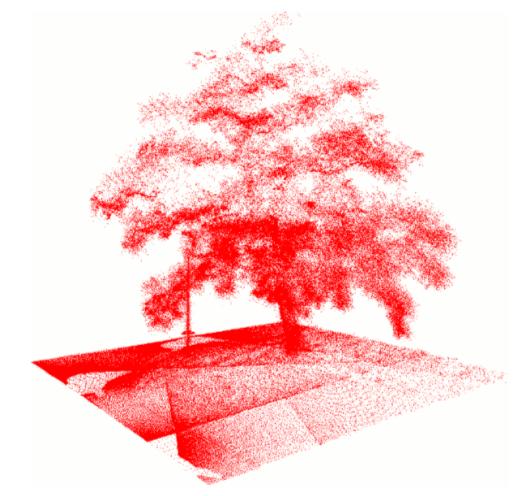
\includegraphics[width=0.8\textwidth]{point_cloud_tree.png}
    % \caption{Awesome Image}
    % \label{fig:awesome_image}
\end{figure}
\end{column}
\end{columns}
\end{frame}

% Voxel Grids

\section{Voxel Grids}

\begin{frame}{Voxel Grids}
\begin{columns}
\begin{column}{0.50\textwidth}
  \begin{block}{\textcolor{green}{Достоинства}}
    \begin{itemize}
    \item
    { 
      Явное представление свободных, занятых и неизвестных областей.
    }
    \item
    {
      Быстрый доступ к элементам.
    }
    \item
    {
      Итеративное обновление, имеющее веротностную интерпретацию.
    }
    \end{itemize}
  \end{block}

  \begin{block}{\textcolor{red}{Недостатки}}
    \begin{itemize}
    \item
    { 
      Требует (ОЧЕНЬ) много памяти.
    }
    \item
    {
      Ошибки дискретизации.
    }
    \end{itemize}
  \end{block}
\end{column}
\begin{column}{0.50\textwidth}
\begin{figure}[h]
    \centering
    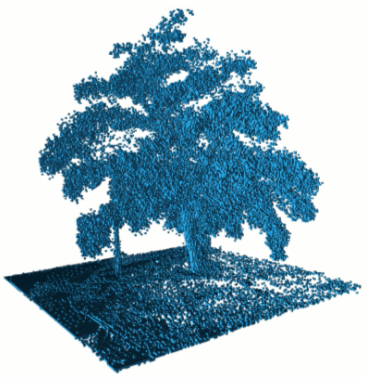
\includegraphics[width=0.8\textwidth]{octomap_tree.png}
    % \caption{Awesome Image}
    % \label{fig:awesome_image}
\end{figure}
\end{column}
\end{columns}
\end{frame}

% Elevation Map

\section{Elevation Map}

\subsection{Elevation Map}


\begin{frame}{Elevation Map}
  Elevation Map - двумерный массив, который в каждой клетке хранит среднее значение высоты и дисперсию.
  Для обновления карты используется фильтр Калмана.

  \begin{figure}[h]
    \centering
    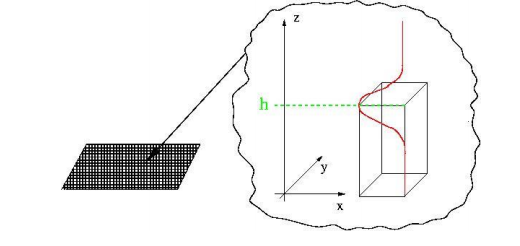
\includegraphics[width=0.8\textwidth]{elev_m_grid.png}
    % \caption{Awesome Image}
    % \label{fig:awesome_image}
  \end{figure}
\end{frame}

\begin{frame}{Elevation Map}
\begin{columns}
\begin{column}{0.50\textwidth}
  \begin{block}{\textcolor{green}{Достоинства}}
    \begin{itemize}
    \item
    { 
      Кушает мало памяти. 2.5D представление окружения
    }
    \item
    {
      Быстрый доступ к элементам.
    }
    \item
    {
      Вероятностная интерпретация.
    }
    \end{itemize}
  \end{block}

  \begin{block}{\textcolor{red}{Недостатки}}
    \begin{itemize}
    \item
    { 
      Одноуровневая карта. Нет явного разделения на свободные, занятые и неизвестные области.
    }
    \item
    {
      Ошибки дискретизации. Не всегда адекватно представляет реальное окружение, что делает её применимой не во всех задачах.
    }
    \end{itemize}
  \end{block}
\end{column}
\begin{column}{0.50\textwidth}
\begin{figure}[h]
    \centering
    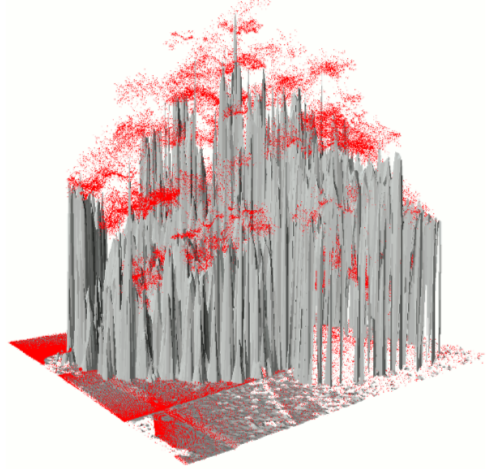
\includegraphics[width=0.8\textwidth]{elev_tree.png}
    % \caption{Awesome Image}
    % \label{fig:awesome_image}
\end{figure}
\end{column}
\end{columns}
\end{frame}

\subsection{Пример Elevation Map}

\begin{frame}{Пример Elevation Map}

\begin{figure}[h]
    \centering
    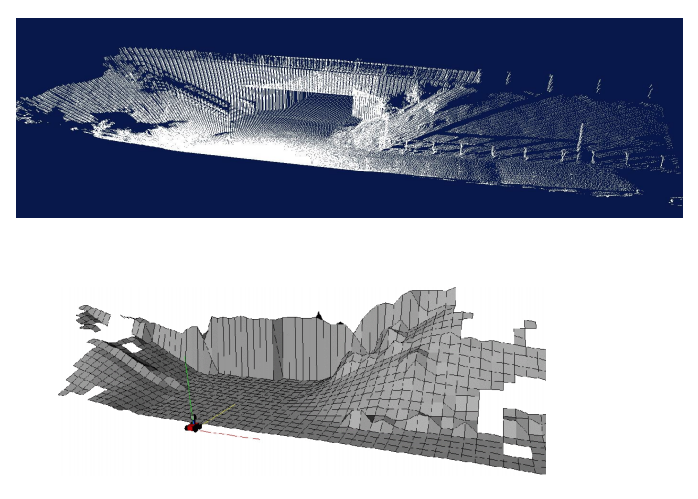
\includegraphics[width=0.8\textwidth]{elev_ex.png}
    % \caption{Awesome Image}
    % \label{fig:awesome_image}
\end{figure}

\end{frame}

% MLS Map
\section{MLS Map}

\subsection{MLS Map}

\begin{frame}{MLS Map}
\begin{columns}
    \begin{column}{0.50\textwidth}
      MLS Map - улучшение Elevation Map.

      В каждой клетке $(i,j)$ хранится список патчей $[P_{ij}^{k}]$.
      Каждый патч состоит из
      \begin{itemize}
        \item
        { 
          Значение средней высоты $\mu$.
        }
        \item
        {
          Дисперсия $\sigma^2$.
        }
        \item
        {
          Глубина $d$.
        }
      \end{itemize}
    \end{column}
    \begin{column}{0.50\textwidth}
      \begin{figure}[h]
        \centering
        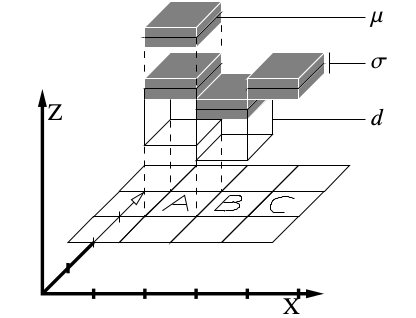
\includegraphics[width=0.9\textwidth]{mls_str.png}
          % \caption{Awesome Image}
          % \label{fig:awesome_image}
      \end{figure}
    \end{column}
  \end{columns}
\end{frame}

\subsection{Создание MLS Map}

\begin{frame}{Создание MLS Map}
  Создание MLS Map состоит из следующих шагов:
  \begin{itemize}
    \item
    { 
      Каждая клетка $(i,j)$ собирает все высоты $z$ точек $p = (x,y,z, \sigma)$ такие, что 
      $si \leq x \leq s(i+1)$ и $sj \leq y \leq s(j+1)$, где $s$ -- ширина клетки.
    }
    \item
    {
      Затем в каждой клетке формируется множество \textcolor{green}{высотных интервалов}. 
      Если разность двух высот не превосходит величины $\gamma$, то эти высоты будут лежать в одном интервале.
      % Из этого следует, что гарантированное расстояние между двумя интервалами будет не меньше $\gamma$.
    }
    \item
    {
      Затем интервалы классифицируются на \textcolor{green}{горизонтальные и вертикальные} по длине интервала. 
      Если она превышает $\tau =$ 10см, то интервал калссифицируется как вертикальный, иначе горизонтальный.
    }
    \end{itemize}
\end{frame}

\begin{frame}{Создание MLS Map}
  \begin{itemize}
    \item
    { 
      Для вертикальных итервалов значениям $\mu$ и $\sigma$ присваивается самое высокое значение интервала, а величине $d$ - длина интервала. Остальные точки удаляются.
    }
    \item
    {
      Для горизонтальных итервалов $\mu$ и $\sigma$ вычисляются через фильтр Калмана, а величина $d = 0$. Все остальное удаляется
    }
    \end{itemize}
\end{frame} 

\subsection{Обновление MLS Map}

\begin{frame}{Обновление MLS Map}
 Обновление состоит из следующих шагов:
  \begin{itemize}
    \item
    { 
      При добавлении новой точки $p=(x,y,z, \sigma)$, находим клетку, в которой эта точка лежит.
    }
    \item
    {
      Затем находим ближайшую по высоте точку. 
      \begin{itemize}
        \item
        { 
          Если оказывается, что новая точка достаточно близка, то происходит процесс обновления $\mu$ и $\sigma$.
        }
        \item
        {
          Если она лежит внутри интервала - ничего не делаем
        }
        \item
        {
          Иначе - добавляем новый патч.
        }
      \end{itemize}
    }
  \end{itemize}
\end{frame}

\subsection{MLS Map}

\begin{frame}{MLS Map}
\begin{columns}
\begin{column}{0.50\textwidth}
  \begin{block}{\textcolor{green}{Достоинства}}
    \begin{itemize}
    \item
    { 
      В одной клетке может храниться несколько уровней
    }
    \end{itemize}
  \end{block}

  \begin{block}{\textcolor{red}{Недостатки}}
    \begin{itemize}
    \item
    {
      Ошибки дискретизации.
    }
    \item
    { 
      Нет явного разделения на свободные, занятые и неизвестные области.
    }
    \item
    {
      Локализация на такой карте - не простая задача.
    }
    \end{itemize}
  \end{block}
\end{column}
\begin{column}{0.50\textwidth}
    \begin{figure}[h]
      \centering
      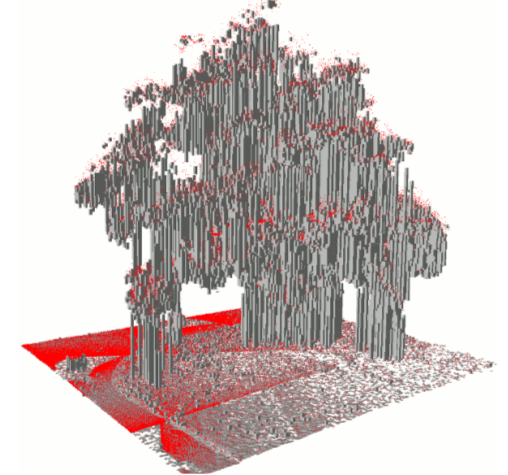
\includegraphics[width=0.9\textwidth]{mls_tree.png}
    % \caption{Awesome Image}
    % \label{fig:awesome_image}
    \end{figure}
\end{column}
\end{columns}
\end{frame}

\subsection{Пример MLS Map}
\begin{frame}{Пример MLS Map}

\begin{figure}[h]
    \centering
    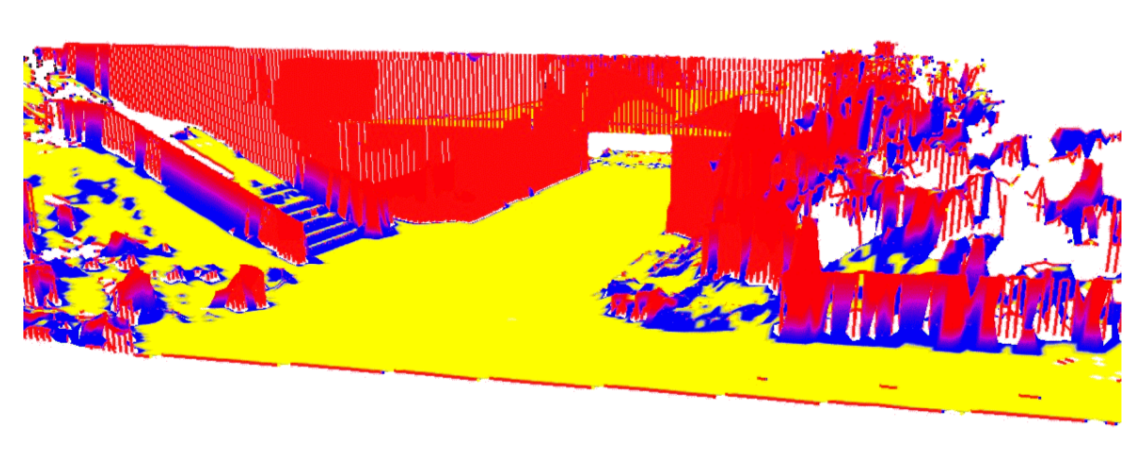
\includegraphics[width=0.65\textwidth]{mls_m.png}
    % \caption{Awesome Image}
    % \label{fig:awesome_image}
\end{figure}

Размер клеток 10см$\times$10см

За 172 скана было нсобрано $45,139,000$ точек, размер территории 299м $\times$ 147м

Объем занятой памяти 73.33 MB.

\begin{figure}[h]
    \centering
    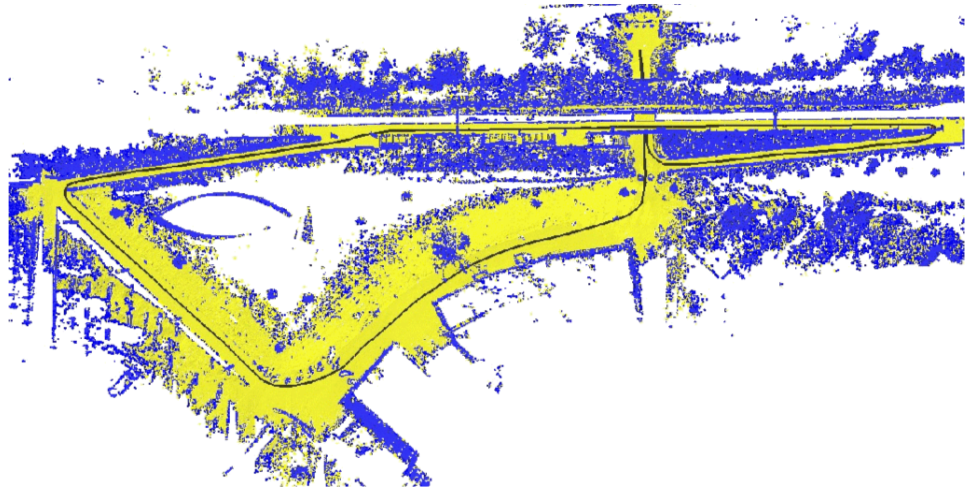
\includegraphics[width=0.65\textwidth]{mls_g.png}
    % \caption{Awesome Image}
    % \label{fig:awesome_image}
\end{figure}


\end{frame}

\section{OctoMap}

\subsection{Octree}
\begin{frame}{Octree}
  \begin{columns}
    \begin{column}{0.50\textwidth}
      \begin{itemize}
        \item
        {
          Древовидная структура.
        }
        \item
        {
          Можно варьировать уровень дискретизации.
        }
        \item
        {
          Память выделяется только когда нужна.
        }
        \item
        {
          А когда нужно, можно дерево сокращать.
        }
      \end{itemize}
    \end{column}
    \begin{column}{0.40\textwidth}
      \begin{figure}[h]
        \centering
        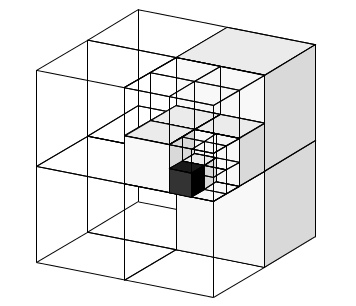
\includegraphics[width=0.8\textwidth]{octree_cube.png}
      \end{figure}

      \begin{figure}[h]
        \centering
        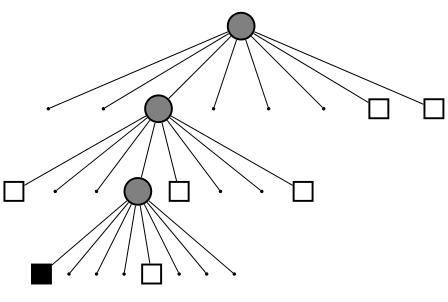
\includegraphics[width=0.8\textwidth]{octree_tree.png}
      \end{figure}
    \end{column}
  \end{columns}  
\end{frame}

\subsection{OctoMap}

\begin{frame}{OctoMap}
  \begin{columns}
    \begin{column}{0.50\textwidth}
        \begin{block}{\textcolor{green}{Достоинства}}
          \begin{itemize}
          \item
          { 
            Полноценное 3D представление окружения.
          }
          \item
          { 
            Вероятностная интерпретация.
          }
          \item
          { 
            Multi-Resolution.
          }
          \item
          { 
            Эффективное использование памяти.
          }
          \end{itemize}
        \end{block}

        \begin{block}{\textcolor{red}{Недостатки}}
          \begin{itemize}
          \item
          {
            Ошибки дискретизации.
          }
          \end{itemize}
        \end{block}
    \end{column}
    \begin{column}{0.40\textwidth}
        \begin{figure}[h]
          \centering
          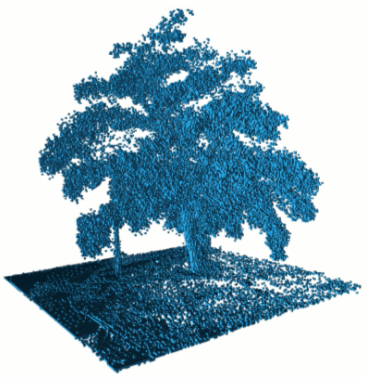
\includegraphics[width=0.8\textwidth]{octomap_tree.png}
          % \caption{Awesome Image}
          % \label{fig:awesome_image}
        \end{figure}
    \end{column}
  \end{columns}  
\end{frame}


\subsection{Обновление OctoMap}

\begin{frame}{Обновление OctoMap}
  Для обновления карты исользуется следующая формула
  $$P(m^{cell}| z_{1..t}) = \left(1 + \frac{1- P(m^{cell} | z_{t})}{P(m^{cell} | z_{t})}  \frac{P(m^{cell})}{1 - P(m^{cell})} 
   \frac{1- P(m^{cell} | z_{1..t-1})} {P(m^{cell} | z_{1..t-1})}\right)^{-1}$$

  Используя обозначение 
  $$L(m^{cell})= \log{ \frac{P(m^{cell})}{1 - P(m^{cell})} }$$
  Получаем
  $$L(m^{cell}| z_{1..t})= L(m^{cell} | z_t) + L(m^{cell} | z_{1..t-1}) - L(m^{cell})$$

\end{frame}

\subsection{Обновление OctoMap}

\begin{frame}{OctoMap}
  \begin{itemize}
  \item
  {
    Ограничие $L(m^{cell}| z_{1..t})$ -- для использования в динамическом окружении и для сокращения дерева
    $$L(m^{cell}| z_{1..t}) = \max( \min(L(m^{cell}| z_{1..t}), l_{max}), l_{min})$$
    $$L(m^{cell}| z_{1..t}) \in (l_{min}, l_{max})$$
  }
  \item
  {
    Можно динамически менять точность карты
    $$L(m^{cell}| z_{1..t}) = \max_{i}{L(m_{i}^{cell}| z_{1..t})}$$
  }
  \end{itemize}
  \begin{figure}[h]
    \centering
    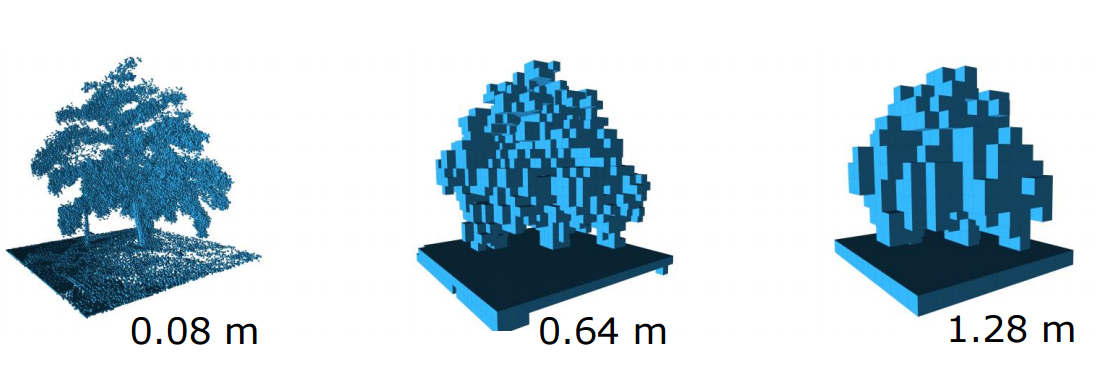
\includegraphics[width=0.8\textwidth]{octomap_multi_res.png}
    % \caption{Awesome Image}
    % \label{fig:awesome_image}
  \end{figure}
\end{frame}

\subsection{Примеры OctoMap}

\begin{frame}{Примеры OctoMap}

Кампус Фрайбургского университета - 292 м $\times$ 167 м $\times$ 28 м 

Voxel Grids - 5162.90 MB 

OctoMap - 379.70 MB

Lossy OctoMap - 13.82 MB

\begin{figure}[h]
    \centering
    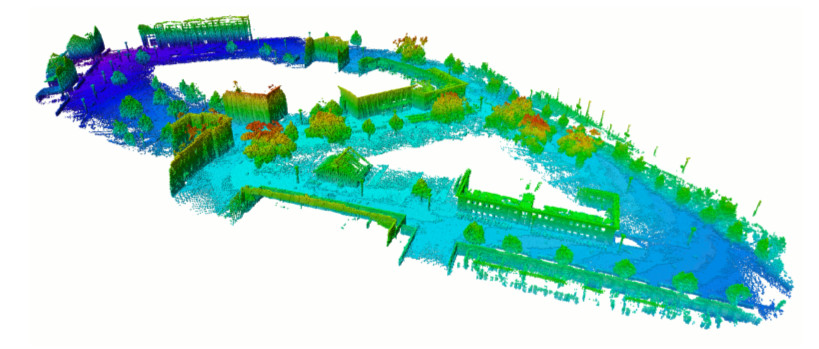
\includegraphics[width=0.8\textwidth]{octomap_fr.png}
    % \caption{Awesome Image}
    % \label{fig:awesome_image}
\end{figure}


\end{frame}

% All of the following is optional and typically not needed. 
\appendix
\section<presentation>*{\appendixname}
\subsection<presentation>*{Источники}

\begin{frame}[allowframebreaks]
  \frametitle<presentation>{Источники}
    
  \begin{thebibliography}{10}
    
  % \beamertemplatebookbibitems
  % Start with overview books.

  \bibitem{ LL }
    Wolfram Burgard, Diego Tipaldi
    \newblock {\url{http://ais.informatik.uni-freiburg.de/teaching/ss15/robotics/slides/17-3dmapping.pdf}}

    \newblock {\em Материалы лекции Фрайбургского университета по курсу Introduction to
    Mobile Robotics - Techniques for 3D Mapping}.
 
  \beamertemplatearticlebibitems
  % Followed by interesting articles. Keep the list short. 

  \bibitem{OctoMap}
    Armin Hornung, Kai M. Wurm, Maren Bennewitz, Cyrill Stachniss, Wolfram Burgard
    \newblock {OctoMap:
  An Efficient Probabilistic 3D Mapping Framework Based on Octrees}
    \newblock {\em Autonomous Robots April 2013, Volume 34, Issue 3, pp 189-206}

  \bibitem{MLS}
    Rudolph Triebel, Patrick Pfaff, Wolfram Burgard
    \newblock {Multi-Level Surface Maps for Outdoor Terrain Mapping and Loop Closing}
    \newblock {\em In Proceedings of the IEEE/RSJ International Conference on Intelligent Robots and Systems (IROS ’06)}

  \end{thebibliography}
\end{frame}

\end{document}


